\documentclass[toc=flat]{scrartcl}

\overfullrule 2pt

\usepackage{lmodern}

\usepackage{booktabs}

\usepackage{tikz}
\usetikzlibrary{automata,positioning}

\usepackage{varioref}
\usepackage{hyperref}
\usepackage{cleveref}

\begin{document}
  \tableofcontents
  
  \section{Regular Expression $\rightarrow$ NFA $\rightarrow$ DFA}
  
  \subsection{Concatenation}
  
  \subsubsection{The regular expression \texttt{//}}
  
  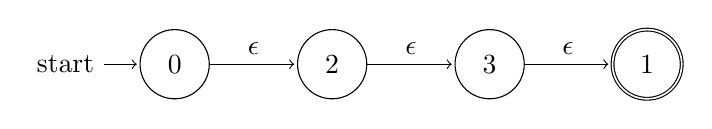
\begin{tikzpicture}[shorten >=1pt,node distance=2cm,on grid,auto]
    \node[state,initial]   (q0)               {$0$};
    \node[state]           (q2) [right=of q0] {$2$};
    \node[state]           (q3) [right=of q2] {$3$};
    \node[state,accepting] (q1) [right=of q3] {$1$};
    
    \path[->] (q0) edge node {$\epsilon$} (q2)
              (q2) edge node {$\epsilon$} (q3)
              (q3) edge node {$\epsilon$} (q1);
  \end{tikzpicture}
  
  \begin{center}
    \begin{tabular}{cc|c}
      \toprule
       & d & $\epsilon$* \\ 
      \midrule
      $\rightarrow$ & 0 & 2,3,1 \\
                    & 2 & 3,1 \\
                    & 3 & 1 \\
      $\leftarrow$  & 1 & --- \\
      \bottomrule
    \end{tabular}
  \end{center}

  Da das Eingabealphabet nach Entfernung von $\epsilon$ leer wird, ist der Automat einfach zu konstruieren.
  
  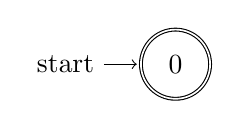
\begin{tikzpicture}[shorten >=1pt,node distance=2cm,on grid,auto]
    \node[state,initial,accepting] (q0) {$0$};
  \end{tikzpicture}
  
  \subsubsection{The regular expression \texttt{/a/}}

  \begin{center}
    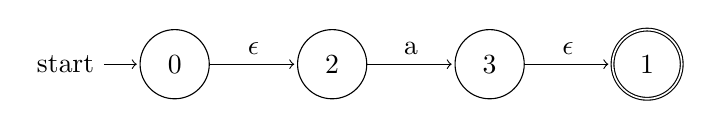
\begin{tikzpicture}[shorten >=1pt,node distance=2cm,on grid,auto]
      \node[state,initial]   (q0)               {$0$};
      \node[state]           (q2) [right=of q0] {$2$};
      \node[state]           (q3) [right=of q2] {$3$};
      \node[state,accepting] (q1) [right=of q3] {$1$};
      
      \path[->] (q0) edge node {$\epsilon$} (q2)
                (q2) edge node {a}          (q3)
                (q3) edge node {$\epsilon$} (q1);
    \end{tikzpicture}
  \end{center}
  
  \begin{center}
    \begin{tabular}{cc|cc}
      \toprule
      & d & a & $\epsilon$* \\ 
      \midrule
      $\rightarrow$ & 0 & --- &   2 \\
                    & 2 &   3 & --- \\
                    & 3 & --- &   1 \\
      $\leftarrow$  & 1 & --- & --- \\
      \bottomrule
    \end{tabular}
  \end{center}
  
  \begin{center}
    \begin{tabular}{cc|c|l}
      \toprule
      & d & a$\epsilon$* & Kommentar \\
      \midrule
      $\rightarrow$ &   0 & --- & eliminieren\\
      $\rightarrow$ &   2 & 3,1 & \\
      $\leftarrow$  & 3,1 & --- & \\
      \bottomrule
    \end{tabular}
  \end{center}
  
  \begin{center}
    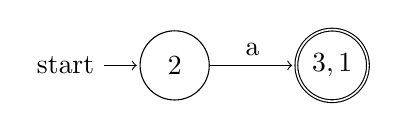
\begin{tikzpicture}[shorten >=1pt,node distance=2cm,on grid,auto]
    \node[state,initial]   (q2)               {$2$};
    \node[state,accepting] (q3) [right=of q2] {$3,1$};
    
    \path[->] (q2) edge node {a}          (q3);
    \end{tikzpicture}
  \end{center}
  
  \subsubsection{The regular expression \texttt{/ab/}}
  
  \begin{center}
    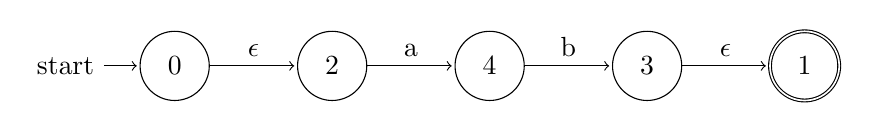
\begin{tikzpicture}[shorten >=1pt,node distance=2cm,on grid,auto]
    \node[state,initial]   (q0)               {$0$};
    \node[state]           (q2) [right=of q0] {$2$};
    \node[state]           (q4) [right=of q2] {$4$};
    \node[state]           (q3) [right=of q4] {$3$};
    \node[state,accepting] (q1) [right=of q3] {$1$};
    
    \path[->] (q0) edge node {$\epsilon$} (q2)
              (q2) edge node {a}          (q4)
              (q4) edge node {b}          (q3)
              (q3) edge node {$\epsilon$} (q1);
    \end{tikzpicture}
  \end{center}
  
  \begin{center}
    \begin{tabular}{cc|ccc}
      \toprule
      & d & a & b & $\epsilon$* \\ 
      \midrule
      $\rightarrow$ & 0 & --- & --- &   2 \\
                    & 2 &   4 & --- & --- \\
                    & 4 & --- &   3 & --- \\
                    & 3 & --- & --- &   1 \\
      $\leftarrow$  & 1 & --- & --- & --- \\
      \bottomrule
    \end{tabular}
  \end{center}
  
  \begin{center}
    \begin{tabular}{cc|cc}
      \toprule
      & d & a$\epsilon$* & b$\epsilon$* \\
      \midrule
      $\rightarrow$ &   2 &   4 & --- \\
                    &   4 & --- & 3,1 \\
      $\leftarrow$  & 3,1 & --- & --- \\
      \bottomrule
    \end{tabular}
  \end{center}
  
  \begin{center}
    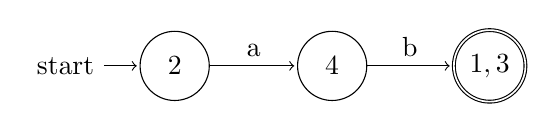
\begin{tikzpicture}[shorten >=1pt,node distance=2cm,on grid,auto]
    \node[state,initial]   (q2)               {$2$};
    \node[state]           (q4) [right=of q2] {4};
    \node[state,accepting] (q3) [right=of q4] {$1,3$};
    
    \path[->] (q2) edge node {a}          (q4)
              (q4) edge node {b}          (q3);
    \end{tikzpicture}
  \end{center}
  
  \subsubsection{The regular expression \texttt{/abc/}}
  
  \begin{center}
    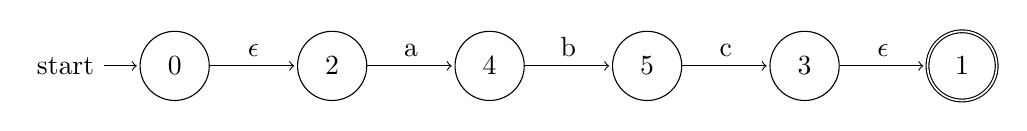
\begin{tikzpicture}[shorten >=1pt,node distance=2cm,on grid,auto]
    \node[state,initial]   (q0)               {$0$};
    \node[state]           (q2) [right=of q0] {$2$};
    \node[state]           (q4) [right=of q2] {$4$};
    \node[state]           (q5) [right=of q4] {$5$};
    \node[state]           (q3) [right=of q5] {$3$};
    \node[state,accepting] (q1) [right=of q3] {$1$};
    
    \path[->] (q0) edge node {$\epsilon$} (q2)
              (q2) edge node {a}          (q4)
              (q4) edge node {b}          (q5)
              (q5) edge node {c}          (q3)
              (q3) edge node {$\epsilon$} (q1);
    \end{tikzpicture}
  \end{center}
  
  \begin{center}
    \begin{tabular}{cc|cccc}
      \toprule
      & d & a & b & c & $\epsilon$* \\ 
      \midrule
      $\rightarrow$ & 0 & --- & --- & --- &   2 \\
                    & 2 &   4 & --- & --- & --- \\
                    & 4 & --- &   5 & --- & --- \\
                    & 5 & --- & --- &   3 & --- \\
                    & 3 & --- & --- & --- &   1 \\
      $\leftarrow$  & 1 & --- & --- & --- & --- \\
      \bottomrule
    \end{tabular}
  \end{center}
  
  \begin{center}
    \begin{tabular}{cc|ccc}
      \toprule
      & d & a$\epsilon$* & b$\epsilon$* & c$\epsilon$* \\
      \midrule
      $\rightarrow$ & 0,2 &   4 & --- & --- \\
                    &   4 & --- &   5 & --- \\
                    &   5 & --- & --- & 3,1 \\
      $\leftarrow$  & 3,1 & --- & --- & --- \\
      \bottomrule
    \end{tabular}
  \end{center}
  
  \begin{center}
    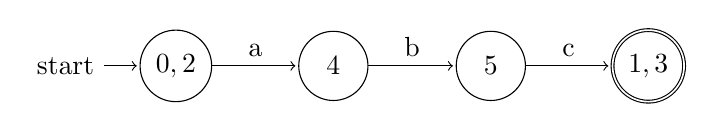
\begin{tikzpicture}[shorten >=1pt,node distance=2cm,on grid,auto]
    \node[state,initial]   (q02)                {$0,2$};
    \node[state]           (q4)  [right=of q02] {$4$};
    \node[state]           (q5)  [right=of q4]  {$5$};
    \node[state,accepting] (q13) [right=of q5]  {$1,3$};
    
    \path[->] (q02) edge node {a}          (q4)
              (q4)  edge node {b}          (q5)
              (q5)  edge node {c}          (q13);
    \end{tikzpicture}
  \end{center}
  
  \subsection{Unions}
  
  \subsubsection{The regular expression \texttt{/|a/}}\label{regex:epsilon-or-a}

  \begin{center}
    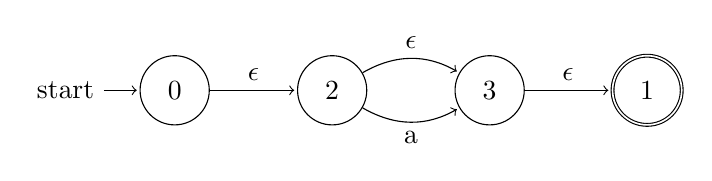
\begin{tikzpicture}[shorten >=1pt,node distance=2cm,on grid,auto]
      \node[state,initial]   (q0)               {$0$};
      \node[state]           (q2) [right=of q0] {$2$};
      \node[state]           (q3) [right=of q2] {$3$};
      \node[state,accepting] (q1) [right=of q3] {$1$};
      
      \path[->] (q0) edge              node         {$\epsilon$} (q2)
                (q2) edge [bend left]  node         {$\epsilon$} (q3)
                (q2) edge [bend right] node [below] {a}          (q3)
                (q3) edge              node         {$\epsilon$} (q1);
    \end{tikzpicture}
  \end{center}
  
  \begin{center}
    \begin{tabular}{cc|cc}
      \toprule
                    & d &   a & $\epsilon$* \\ 
      \midrule
      $\rightarrow$ & 0 & --- & 1,2,3 \\
                    & 2 &   3 &   1,3 \\
                    & 3 & --- &     1 \\
      $\leftarrow$  & 1 & --- &   --- \\
      \bottomrule
    \end{tabular}
  \end{center}
  
  \begin{center}
    \begin{tabular}{cc|c}
      \toprule
                                   &   d   & a$\epsilon$* \\
       \midrule
       $\rightarrow$, $\leftarrow$ & 1,2,3 & 1,3 \\
       $\leftarrow$                &  1,3  & --- \\
       \bottomrule
    \end{tabular}
  \end{center}
  
  \begin{center}
    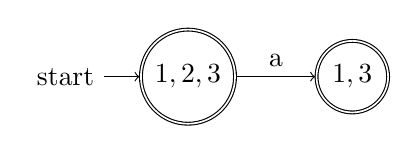
\begin{tikzpicture}
      \node[state,initial,accepting] (q123)                 {$1,2,3$};
      \node[state,accepting]         (q13)  [right=of q123] {$1,3$};
      
      \path[->] (q123) edge node [above] {a} (q13);
    \end{tikzpicture}
  \end{center}
  
  \subsubsection{The regular expression \texttt{/|a/}}
  
  The construction is similar to \vref{regex:epsilon-or-a}.
  
  \subsubsection{The regular expression \texttt{/a|b/}}
  
  \begin{center}
    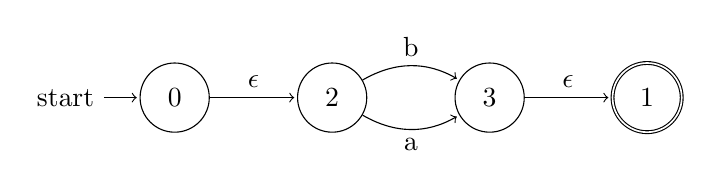
\begin{tikzpicture}[shorten >=1pt,node distance=2cm,on grid,auto]
    \node[state,initial]   (q0)               {$0$};
    \node[state]           (q2) [right=of q0] {$2$};
    \node[state]           (q3) [right=of q2] {$3$};
    \node[state,accepting] (q1) [right=of q3] {$1$};
    
    \path[->] (q0) edge              node         {$\epsilon$} (q2)
              (q2) edge [bend left]  node         {b}          (q3)
              (q2) edge [bend right] node [below] {a}          (q3)
              (q3) edge              node         {$\epsilon$} (q1);
    \end{tikzpicture}
  \end{center}
  
  \begin{center}
    \begin{tabular}{cc|ccc}
      \toprule
                    & d &   a &   b & $\epsilon$* \\ 
      \midrule
      $\rightarrow$ & 0 & --- & --- &   2 \\
                    & 2 &   3 &   3 & --- \\
                    & 3 & --- & --- &   1 \\
      $\leftarrow$  & 1 & --- & --- & --- \\
      \bottomrule
    \end{tabular}
  \end{center}
  
  \begin{center}
    \begin{tabular}{cc|cc}
      \toprule
                    &   d & a$\epsilon$*  & b$\epsilon$* \\
      \midrule
      $\rightarrow$ &   2 & 1,3 & 1,3 \\
      $\leftarrow$  & 1,3 & --- & --- \\
      \bottomrule
    \end{tabular}
  \end{center}
  
  \begin{center}
    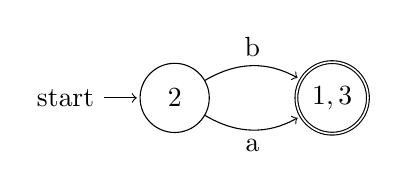
\begin{tikzpicture}[shorten >=1pt,node distance=2cm,on grid,auto]
    \node[state,initial]   (q2)               {$2$};
    \node[state,accepting] (q13) [right=of q2] {$1,3$};
    
    \path[->] (q2) edge [bend left]  node         {b} (q13)
              (q2) edge [bend right] node [below] {a} (q13);
    \end{tikzpicture}
  \end{center}
  
  \subsubsection{The regular expression \texttt{/ab|c/}}\label{regex:ab-or-c}
  
  \begin{center}
    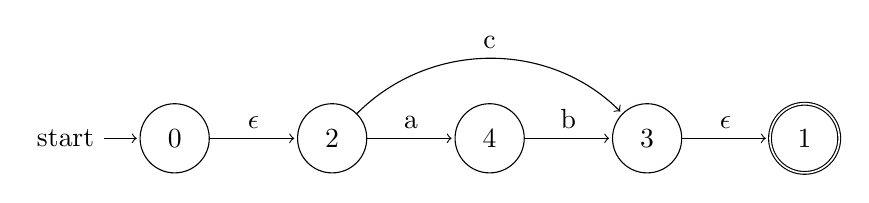
\begin{tikzpicture}[shorten >=1pt,node distance=2cm,on grid,auto]
      \node[state,initial]   (q0)                     {$0$};
      \node[state]           (q2) [right=of q0]       {$2$};
      \node[state]           (q4) [right=of q2] {$4$};
      \node[state]           (q3) [right=of q4]     {$3$};
      \node[state,accepting] (q1) [right=of q3]       {$1$}; 
    
      \path[->] (q0)                edge node {$\epsilon$} (q2)
                (q2)                edge node {a}          (q4)
                (q4)                edge node {b}          (q3)
                (q2) [bend left=45] edge node {c}          (q3)
                (q3) [bend left=0]  edge node {$\epsilon$} (q1);
    \end{tikzpicture}
  \end{center}
  
  \begin{center}
    \begin{tabular}{cc|cccc}
       \toprule
                     & d &   a &   b & c   & $\epsilon$* \\
       \midrule
       $\rightarrow$ & 0 & --- & --- & --- &   2 \\
                     & 2 &   4 & --- &   3 & --- \\
                     & 3 & --- & --- & --- &   1 \\
                     & 4 & --- &   3 & --- & --- \\
       $\leftarrow$  & 1 & --- & --- & --- & --- \\
       \bottomrule
    \end{tabular}
  \end{center}
  
  \begin{center}
    \begin{tabular}{cc|ccc}
      \toprule
                    & d & a$\epsilon$*  & b$\epsilon$* & c$\epsilon$* \\
      \midrule
      $\rightarrow$ &  2  &  4  & --- & 1,3 \\
                    &  4  & --- & 1,3 & --- \\
      $\leftarrow$  & 1,3 & --- & --- & --- \\
    \end{tabular}
  \end{center}
  
  \begin{center}
    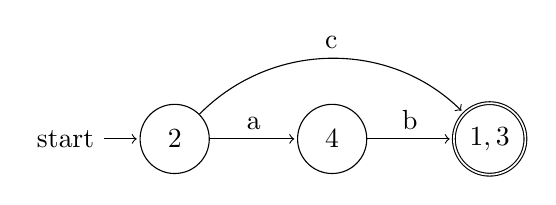
\begin{tikzpicture}[shorten >=1pt,node distance=2cm,on grid,auto]
      \node[state,initial]   (q2)                {$2$};
      \node[state]           (q4)  [right=of q2] {$4$};
      \node[state,accepting] (q13) [right=of q4] {$1,3$};
      
      \path[->] (q2)                edge node {a} (q4)
                (q4)                edge node {b} (q13)
                (q2) [bend left=45] edge node {c} (q13);
    \end{tikzpicture}
  \end{center}
  
  \subsubsection{The regular expression \texttt{/a|bc/}}
  
  The construction should be very similar to \vref{regex:ab-or-c}, except for the names of the states and edges.
  
  \subsection{Repeat 0 or more (*)}
  
  \subsubsection{The regular expression \texttt{/a*/}}
  
  \begin{center}
    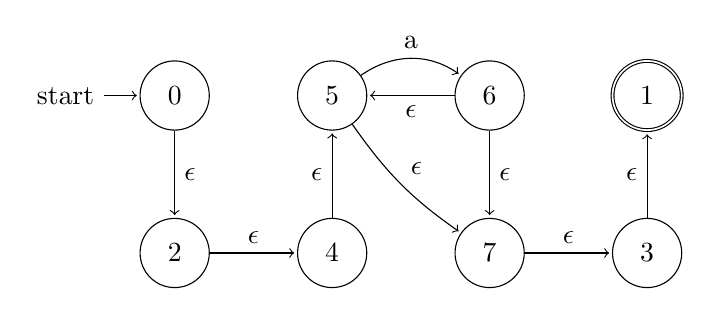
\begin{tikzpicture}[shorten >=1pt,node distance=2cm,on grid,auto]
      \node[state,initial]   (q0)               {$0$};
      \node[state]           (q2) [below=of q0] {$2$};
      \node[state]           (q4) [right=of q2] {$4$};
      \node[state]           (q5) [above=of q4] {$5$};
      \node[state]           (q6) [right=of q5] {$6$};
      \node[state]           (q7) [below=of q6] {$7$};
      \node[state]           (q3) [right=of q7] {$3$};
      \node[state,accepting] (q1) [above=of q3] {$1$};
      
      \path[->] (q0)                 edge node {$\epsilon$} (q2)
                (q2)                 edge node {$\epsilon$} (q4)
                (q4)                 edge node {$\epsilon$} (q5)
                (q5) [bend left=35]  edge node {a}          (q6)
                (q6) [bend left=0]   edge node {$\epsilon$} (q5)
                (q5) [bend right=10] edge node {$\epsilon$} (q7)
                (q6) [bend left=0]   edge node {$\epsilon$} (q7)
                (q7)                 edge node {$\epsilon$} (q3)
                (q3)                 edge node {$\epsilon$} (q1);
    \end{tikzpicture}
  \end{center}
  
\end{document}